 \documentclass[11pt]{article} 
\usepackage[english]{babel}
\usepackage[utf8]{inputenc}
\usepackage[margin=0.5in]{geometry}
\usepackage{amsmath}
\usepackage{amsthm}
\usepackage{amsfonts}
\usepackage{amssymb}
\usepackage[usenames,dvipsnames]{xcolor}
\usepackage{graphicx}
\usepackage[siunitx]{circuitikz}
\usepackage{tikz}
\usepackage[colorinlistoftodos, color=orange!50]{todonotes}
\usepackage{hyperref}
\usepackage[numbers, square]{natbib}
\usepackage{fancybox}
\usepackage{epsfig}
\usepackage{soul}
\usepackage[framemethod=tikz]{mdframed}
\usepackage[shortlabels]{enumitem}
\usepackage[version=4]{mhchem}
\usepackage{multicol}

\usepackage{mathtools}
\usepackage{comment}
\usepackage{enumitem}
\usepackage[utf8]{inputenc}
\usepackage[linesnumbered,ruled,vlined]{algorithm2e}
\usepackage{listings}
\usepackage{color}
\usepackage[numbers]{natbib}
\usepackage{subfiles}
\usepackage{tkz-berge}


\newtheorem{prop}{Proposition}[section]
\newtheorem{thm}{Theorem}[section]
\newtheorem{lemma}{Lemma}[section]
\newtheorem{cor}{Corollary}[prop]

\theoremstyle{definition}
\newtheorem{definition}{Definition}

\theoremstyle{definition}
\newtheorem{required}{Problem}

\theoremstyle{definition}
\newtheorem{ex}{Example}


\setlength{\marginparwidth}{3.4cm}
%#########################################################

%To use symbols for footnotes
\renewcommand*{\thefootnote}{\fnsymbol{footnote}}
%To change footnotes back to numbers uncomment the following line
%\renewcommand*{\thefootnote}{\arabic{footnote}}

% Enable this command to adjust line spacing for inline math equations.
% \everymath{\displaystyle}

% _______ _____ _______ _      ______ 
%|__   __|_   _|__   __| |    |  ____|
%   | |    | |    | |  | |    | |__   
%   | |    | |    | |  | |    |  __|  
%   | |   _| |_   | |  | |____| |____ 
%   |_|  |_____|  |_|  |______|______|
%%%%%%%%%%%%%%%%%%%%%%%%%%%%%%%%%%%%%%%

\title{
\normalfont \normalsize 
\textsc{CSCI 3104 Spring 2022 \\ 
Instructors: Profs. Chen and Layer} \\
[10pt] 
\rule{\linewidth}{0.5pt} \\[6pt] 
\huge Quiz 7 -- Safe and useless edges \\
\rule{\linewidth}{2pt}  \\[10pt]
}
%\author{Your Name}
\date{}

\begin{document}
\definecolor {processblue}{cmyk}{0.96,0,0,0}
\definecolor{processred}{rgb}{200, 0, 0}
\definecolor{processgreen}{rgb}{0, 255, 0}
\DeclareGraphicsExtensions{.png}
\DeclareGraphicsExtensions{.gif}
\DeclareGraphicsExtensions{.jpg}

\maketitle


%%%%%%%%%%%%%%%%%%%%%%%%%
%%%%%%%%%%%%%%%%%%%%%%%%%%
%%%%%%%%%%FILL IN YOUR NAME%%%%%%%
%%%%%%%%%%AND STUDENT ID%%%%%%%%
%%%%%%%%%%%%%%%%%%%%%%%%%%
\noindent
Due Date \dotfill February 18 \\
Name \dotfill \textbf{Julia Troni} \\
Student ID \dotfill \textbf{109280095} \\

\tableofcontents

\section{Instructions}
 \begin{itemize}
	\item The solutions \textbf{should be typed}, using proper mathematical notation. We cannot accept hand-written solutions. \href{http://ece.uprm.edu/~caceros/latex/introduction.pdf}{Here's a short intro to \LaTeX.}
	\item You should submit your work through the \textbf{class Canvas page} only. Please submit one PDF file, compiled using this \LaTeX \ template.
	\item You may not need a full page for your solutions; pagebreaks are there to help Gradescope automatically find where each problem is. Even if you do not attempt every problem, please submit this document with no fewer pages than the blank template (or Gradescope has issues with it).

	\item You \textbf{may not collaborate with other students}. \textbf{Copying from any source is an Honor Code violation. Furthermore, all submissions must be in your own words and reflect your understanding of the material.} If there is any confusion about this policy, it is your responsibility to clarify before the due date. 

	\item Posting to \textbf{any} service including, but not limited to Chegg, Discord, Reddit, StackExchange, etc., for help on an assignment is a violation of the Honor Code.

\end{itemize}


\newpage
\section{Standard 6- Safe and Useless Edges}

\subsection{Problem \ref{Safe1}}
\begin{required} \label{Safe1}
Consider the following graph $G(V, E, w)$. Suppose we have the intermediate spanning forest $\mathcal{F}$ (indicated using thick edges) consisting of the edges $\{A, B\}$, $\{A, C\}$, and $\{D, E\}$. Clearly identify the safe, useless, and undecided edges. Justify your reasoning. 
\begin{center}
\begin {tikzpicture}[semithick]
\tikzstyle{blue}=[circle ,top color =white , bottom color = processblue!20 ,draw,processblue , text=blue , minimum width =1 cm];
\tikzstyle{red}=[circle ,top color =white , bottom color = processred!20 ,draw, processred , text=blue , minimum width =1 cm];
\tikzstyle{green}=[circle ,top color =white , bottom color = processgreen!20 ,draw, processgreen , text=blue , minimum width =1 cm];

	\node[blue] (A) {$A$};
	\node[blue] (B) [above right = of A] {$B$};
	\node[blue] (C) [below right = of A] {$C$};
	\node[blue] (D) [right = of B] {$D$};
	\node[blue] (E) [right = of C] {$E$};
	\node[blue] (F) [below right = of D] {$F$};
	
	\draw[line width=3pt]  (A) edge node[above] {$2$} (B);
	\draw[line width=3pt] (A) edge node[right] {$5$} (C);
	\path (B) edge node[left] {$8$} (C);
	\path (B) edge node[above] {$5$} (D);
	\path (C) edge node[above] {$4$} (E);
	\draw[line width=3pt] (E) edge node[right] {$2$} (D);
	\path (D) edge node[above] {$7$} (F);
	\path (E) edge node[below] {$5$} (F);
	\end{tikzpicture}  
\end{center}
\end{required}


\begin{proof}[Answer]
%You may type your answer here if you wish.

 $\{C,E\}$, and $\{E,F\}$ are \textbf{safe} edges with respect to  $\mathcal{F}$ because they are each the minimum weight edges that crosses a partition of the vertices (a cut), so they are each light edges. Since any light edge that connects two components in an intermediate spanning forest is safe, they are safe.  \\
 $\{B,C\}$ is a \textbf{useless} edge with respect to  $\mathcal{F}$ because it would create a cycle \\
$\{B,D\}$, $\{D,F\}$ are \textbf{undecided} edges with respect to  $\mathcal{F}$ because they are neither safe, nor useless \\
\begin{enumerate}
\item $\{C,E\}$ is the minimum weight edge with exactly one endpoint in the the component $\{A,B,C\}$ and the minimum weight edge with exactly one endpoint in the component $\{D,F,E\}$. Therefore $\{C,E\}$ is a light edge and hence a \textbf{safe} edge with respect to  $\mathcal{F}$
\item $\{E,F\}$ is the minimum weight edge with exactly one endpoint in the the component $\{A,B,D,C,E\}$ and the minimum weight edge with exactly one endpoint in the component $\{F\}$. Therefore $\{E,F\}$ is a light edge and hence a \textbf{safe} edge with respect to  $\mathcal{F}$ \\

See below for a visual of the safe edges \\

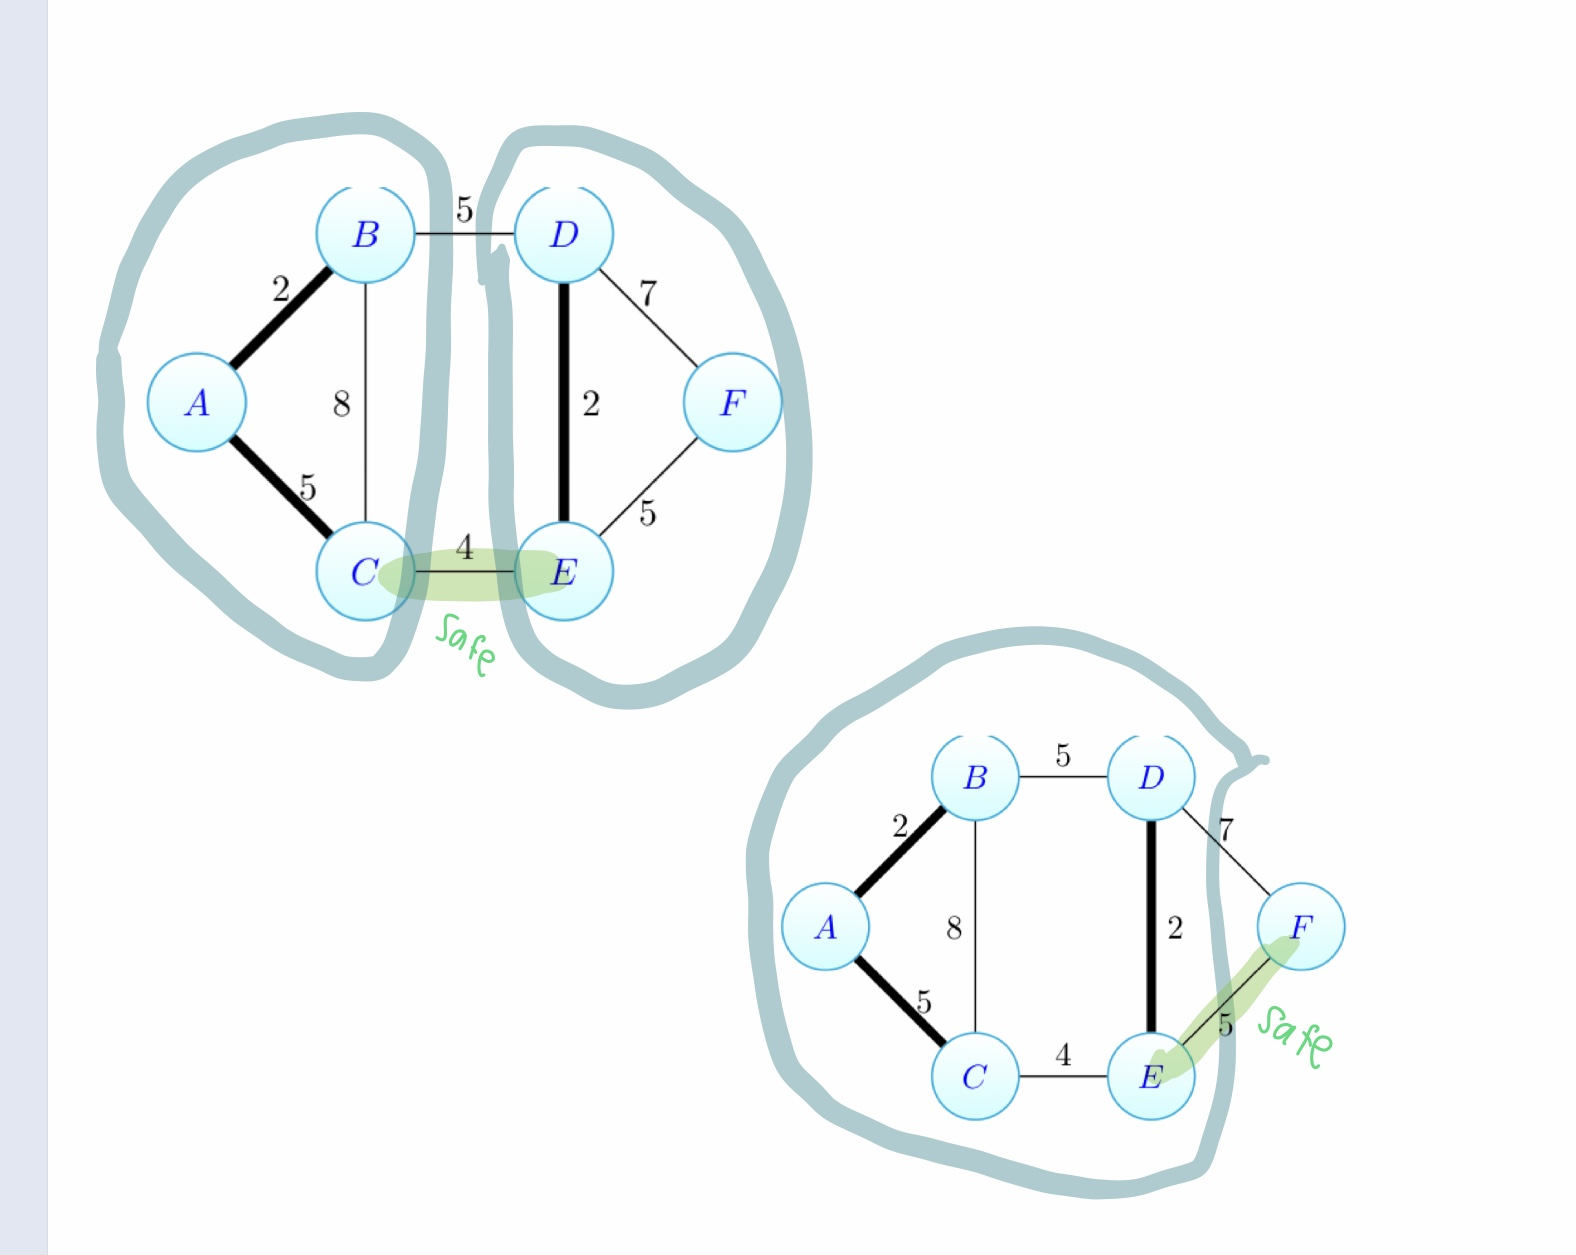
\includegraphics[width=0.7\textwidth]{q7} \\

\item While the edge $\{B,D\}$ hasexactly one endpoint in the the component $\{A,B,C,E,F\}$ and one endpoint in the component $\{D\}$, it is not the minimum weight edge in doing so. Therefore $\{B,D\}$ is an \textbf{undecided} edge with respect to  $\mathcal{F}$
\item While the edge $\{D,F\}$ has exactly one endpoint in the component $\{A,B,C,E,F\}$ and one endpoint in the component $\{D\}$, it is not a minimum weight edge in doing so. Therefore, $\{D,F\}$ is an \textbf{undecided} edge with respect to  $\mathcal{F}$
\item Lastly, the edge $\{B,C\}$ has both endpoints in the component  $\{A,B,C\}$, thus creating a cycle. So $\{B,C\}$ is a \textbf{useless} edge with respect to  $\mathcal{F}$
\end{enumerate}
\end{proof}

% Either type your answer in below, or uncomment the \includegraphics command
% and use it to insert an approprate image. Try experimenting with the scale 
% 0.9 the width option to resize your image if necessary.

%\includegraphics[width=0.9\textwidth]{solution.jpg}


%%%%%%%%%%%%%%%%%%%%%%%%%%%%%%%%%%%%%%%%%%%%%%%%%%
\end{document} % NOTHING AFTER THIS LINE IS PART OF THE DOCUMENT



